%%%%%%%%%%%%%%%%%%%%%%%%%%%%%%%%%%%%%%%%%%%%%%%%%%%%%%%%%%%%%%%%%%%%%%%%%%%%%%%%
%2345678901234567890123456789012345678901234567890123456789012345678901234567890
%        1         2         3         4         5         6         7         8

\documentclass[letterpaper, 10 pt, conference]{ieeeconf}  % Comment this line out if you need a4paper

%\documentclass[a4paper, 10pt, conference]{ieeeconf}      % Use this line for a4 paper

\IEEEoverridecommandlockouts                              % This command is only needed if 
                                                          % you want to use the \thanks command

\overrideIEEEmargins                                      % Needed to meet printer requirements.

% See the \addtolength command later in the file to balance the column lengths
% on the last page of the document

% The following packages can be found on http:\\www.ctan.org
\usepackage{graphics} % for pdf, bitmapped graphics files
\usepackage{epstopdf}
\usepackage{epsfig} % for postscript graphics files
%\usepackage{mathptmx} % assumes new font selection scheme installed
%\usepackage{times} % assumes new font selection scheme installed
\usepackage{amsmath} % assumes amsmath package installed
\usepackage{amssymb}  % assumes amsmath package installed
\DeclareMathOperator{\sgn}{sgn}
\title{\LARGE \bf
Simulation-Driven Robot Controller Design
}


\author{Jie Tan$^{1}$ ~~~Zhaoming Xie$^{1}$ ~~~Byron Boots$^{2}$ ~~~Greg Turk$^{2}$ ~~~Karen Liu$^{2}$% <-this % stops a space
\thanks{$^{1}$The authors are with College of Computing, Georgia Institute of Technology, Atlanta, GA, USA. Email:
        {\tt\small \{jtan34, zxie47\}@gatech.edu}}%
\thanks{$^{2}$The authors are with College of Computing, Georgia Institute of Technology, Atlanta, GA, USA. Email:
        {\tt\small \{bboots, turk, karenliu\}@cc.gatech.edu}}%
}


\begin{document}

\maketitle
\thispagestyle{empty}
\pagestyle{empty}


%%%%%%%%%%%%%%%%%%%%%%%%%%%%%%%%%%%%%%%%%%%%%%%%%%%%%%%%%%%%%%%%%%%%%%%%%%%%%%%%
\begin{abstract}
Many locomotion tasks, such as sit-to-stand, involve changing postures while maintaining balance. Understanding and synthesizing these motions can have fundamental impacts in robotics, but controlling a humanoid robot to perform such motions is challenging. In this paper, we present a system that can automatically design robot controllers for these locomotion tasks. Our system uses simulation and optimization algorithms to find optimal controllers in a physically-simulated environment. It then relies on simulation calibration to transfer the controller from the virtual to the real world. Our experiments show that this system can automatically find successful controllers for a wide variety of locomotion tasks, including lean-to-stand, sit-to-stand, kneel-to-stand and stand-to-handstand.

\end{abstract}

\section{Introduction}

Many of our daily activities involve changing whole-body posture to a target pose without losing balance. For example, to rise from a chair, we carefully maintain balance while switching from a sitting to a standing pose. There are a large variety of motions of similar kind, such as lean-to-stand and kneel-to-stand. Many strategies have been identified to achieve these tasks in biomechanics studies \cite{schenkman:1990,riley:1991,hughes:1994,hughes:1996}. On one end of the spectrum, people employ stabilization strategy in which very little momentum is generated and the center of mass (COM) is constantly supported. In this work, we are interested in the other end of the spectrum, called momentum transfer strategy, in which rapid movements are used to maintain balance even when the COM is outside the support polygon. Studying motions employing momentum transfer strategy can have far-reaching impacts in robotics, especially in rehabilitation, exoskeleton and humanoid robots. 

A robot controller often consists of an open loop reference trajectory and a feedback mechanism. Although careful feedback controls are necessary in the momentum transfer strategy, a trajectory of a purposeful and forceful motion is of great importance. Designing a reference trajectory for these tasks is extremely challenging because achieving these tasks require complex motor skills, delicate balance strategies and rich interactions with the environments. These trajectories are often designed manually by highly-specialized engineers through a time-consuming, trial-and-error process. It involves laborious manual tuning and numerous costly robot experiments. In contrast, our system can design the reference trajectory automatically and requires minimal human intervention. It replaces the tedious manual tuning with automatic optimization processes, and drastically reduces the number of expensive robot experiments. Our system consists of three main components, physical simulation, trajectory optimization and simulation calibration. We first build a \emph{physical simulation} to simulate the dynamics of the robot and its interaction with the environments. We use \emph{trajectory optimization} to search for the optimal trajectory for the task in the simulation. However, even though this optimal trajectory works effectively in the simulation, it can perform poorly on a robot in the real environment. This ``Reality Gap'' \cite{Jakobi95} is caused by various simplifications in simulation algorithms, such as simplified actuator models, inaccurate physical parameters, and ignored hardware limitations, noise and latency. 

We use \emph{simulation calibration} to cross the Reality Gap. Simulation calibration is a dynamic system identification method. We want to emphasize that the goal of simulation calibration is to effectively design reference trajectories that works in the real world, instead of finding the ground truth about the hardware parameters. During calibration, we collect real performance data on the robot, and use it to improve our physical model. Unlike traditional system identification, which is a separate step from controller design, our simulation calibration is tightly coupled with the trajectory optimization. We directly track the optimal trajectory that is found in the simulation to collect real data for system identification. In this way, the simulation is calibrated at the vicinity of the current optimal trajectory. The computation is focused at the important regions of the control space and thus fewer robot experiments are needed. Through calibration, the simulator can capture the real world dynamics more faithfully. This calibrated simulator is used again in trajectory optimization to improve the quality of the controller. We evaluate our system using four tasks: lean-to-stand, sit-to-stand, kneel-to-stand and stand-to-handstand. Although these tasks are distinctively different, our system can find successful reference trajectories for all the tasks automatically.

Our main contribution is the complete pipeline that can automatically design open loop reference trajectories to control a robot to achieve a wide range of tasks. Starting from task specifications, our system can find the trajectories that operate on the robot, with minimal human intervention. This simulation-driven approach effectively cuts the time and the cost of robot controller design. 

\section{Related Work}
\ignorethis{\karen{Ensemble-CIO: Full-body dynamic motion planning that transfers to physical humanoids, Mordatch \etal.}}
The locomotion tasks that this paper foucses on involve changing postures and maintaining balance during the motion. Tasks that fall into this category and are extensively studied in robotics are sit-to-stand \cite{Faloutsos:2003,Iida:2004,Pchelkin:2010,Mistry:2010} and lie-to-stand \cite{morimoto:1998,Faloutsos:2001,Hirukawa:2005,Kanehiro:2007}. While many of these prior work focuses on one specific motion, we target at a more general problem of finding controllers for a wide range of such locomotion tasks. A few related work tried to tackle this more general problem. Jones \cite{jones:2011} developed rising motions for both biped and quadraped using pose tracking, orientation correction and virtual force. Lin and Huang \cite{lin:2012} used motion planning and dynamics filtering to develop rising up motions from various initial lying poses. Tassa et al. \cite{tassa:2012} used Model Predictive Control to synthesize complex behaviors, including getting up from an aribitrary pose on the ground. Although these work has shown impressive results in simulation, experiments on real robots were not presented.

Locomotion often involve frequent change of contacts. It poses significant challenges to controller optimization due to the discontinuous contact forces. We choose to use Covariance Matrix Adaptation (CMA) \cite{Hansen:2009}, a stochastic sampling-based optimization algorithm, to tackle this challenge. Although CMA is not widely used in robotics, it is a popular method in physically-based character animation to search for control parameters when the problem domain is highly discontinous \cite{Wu:2010, Wang:2010, Tan:2014}.

A controller that is designed in simulation may not work in the real environment. This discrepancy of performance is called Reality Gap. One way to cross the reality gap is to improve the simulation model using real data that is measured from robot experiments. Ha and Yamane \cite{HA:2015} performed Gaussian process regression to model the error between the simulated and the real data, and then augmented the simulation with this error model. Abbeel et al. \cite{Abbeel:2006} started from an inaccurate physical model but successively grounded the policy evaluations using real-life trials. Grounded simulated learning approach \cite{Farchy:2013} iteratively optimized the controller, measured the discrepancy and modified the simulator using supervised learning algorithms. Zagal et al. \cite{zagal2004} coevolved the controller and the simulator using genetic algorithms. Mordatch et al. \cite{Mordatch:2015} performed trajectory optimization using ensembles of perturbed physical models, which increased the success rate when the controller was executed on the robot.

Our simulation calibration subsystem narrows down the Reality Gap using off-white dynamic system identification methods \cite{ljung:2010}. A typical dynamic system identification involve experiment design and parameter estimation \cite{swevers:2007}. Experiments could be designed manually or automatically with genetic algorithms \cite{BongardL05}. In locomotion and manipulation related tasks, in which contact changes are frequent, the experiments are usually designed independently from control tasks because the parameters are better inferred with a contact free behavior \cite{Kolev:2015}. As a result, lengthy experiments and huge amount of data are needed in system identification, in the hope that the collected data covers the important regions of the control space. In contrast, our system tightly couples simulation calibration and controller optimization. The current controller that is optimized in the simulation is used as the experiment for system identification. This is made possible by CMA, which can estimate parameters even when contact changes in the experiments. 


\section{Overview}

\begin{figure}[!t]
  \centering
  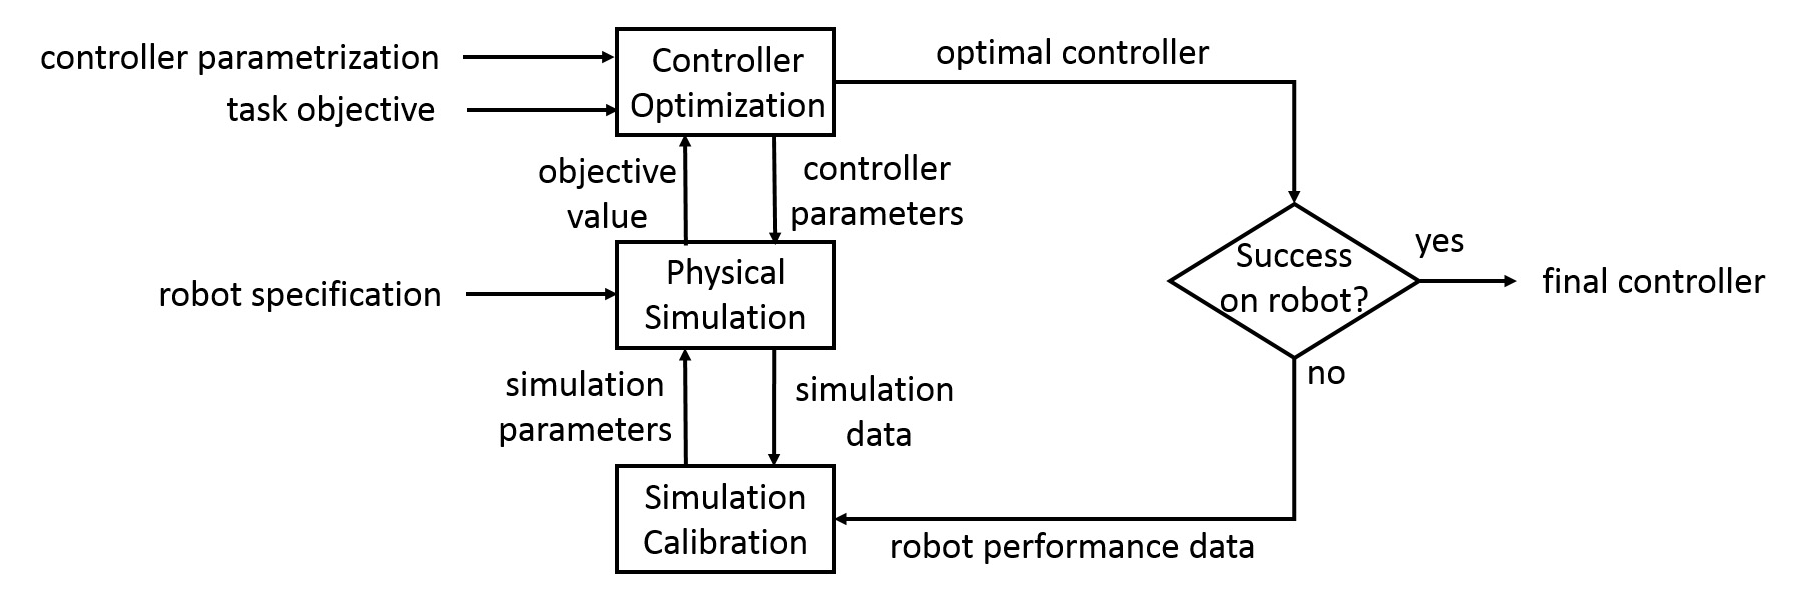
\includegraphics[width=0.5\textwidth]{figures/controllerTransfer}
  \caption{Overview of our algorithm.}
  \vspace{-0.1in}
  \label{fig:controllerTransferOverview}
\end{figure}

We have developed a system that can automatically design reference trajectories for robots to execute transition motions (Figure~\ref{fig:controllerTransferOverview}). Given the specification of the robot, including its body shape, the physical properties of each body, and the types of joints, we build a physical simulation using Dynamic Animation and Robotics Toolkit (DART) \cite{dart:2012}. The trajectory optimization subsystem runs thousands of simulations to search for the optimal trajectory that maximizes the task-related fitness function. We then test this optimal trajectory on the robot. If the robot successfully completes the task, a solution is found and our algorithm terminates. Otherwise, we record the robot performance data and feed it into the simulation calibration subsystem. Simulation calibration runs another optimization, which searches for the optimal simulation parameters to minimize the discrepancy between the performance of the robot in the simulation and in the real world. The loop of trajectory optimization and simulation calibration is performed iteratively until the reference trajectory works successfully on the real robot. In the next three sections, we will present the algorithmic details of these components.

\section{Physical Simulation}

\subsection{Dynamics Equations}

We model the robot as an articulated rigid body system in our simulator. We represent the states of the system $(\mathbf{x}, \dot{\mathbf{x}})$ in generalized coordinates, where $\mathbf{x}$ includes the global position $\mathbf{p}$, the orientation $\mathbf{r}$ of the root body (robot's torso), and the joint angles $\mathbf{q}$. The governing equations of motion is as follow:

\begin{equation}
\label{eq:robotdynamics}
\mathbf{M}(\mathbf{x})\mathbf{\ddot{x}}+\mathbf{C}(\mathbf{x},\mathbf{\dot{x}})=\mathbf{\tau}(\mathbf{q}, \dot{\mathbf{q}}, \bar{\mathbf{q}})+\mathbf{J}^T\mathbf{f}
\end{equation}
where $\mathbf{M}(\mathbf{x})$ is the mass matrix and $\mathbf{C}(\mathbf{x},\mathbf{\dot{x}})$ is the Coriolis and Centrifugal force. $\mathbf{\tau}(\mathbf{q}, \dot{\mathbf{q}}, \bar{\mathbf{q}})$ are joint torques exerted by the actuators, which depends on the current joint angles $\mathbf{q}$, velocities $\dot{\mathbf{q}}$ and desired angles $\bar{\mathbf{q}}$. The relation between these quantities is determined by the actuator model, which is presented in the next section. $\mathbf{J}$ is the Jacobian matrix and $\mathbf{f}$ is the external contact force, which is computed based on linear complementarity conditions \cite{Tan:2012b}. In our implementation, we use DART to solve the contact force and numerically integrate the system state $(\mathbf{x}, \dot{\mathbf{x}})$ over time.

\subsection{Actuator Model}
\label{sec:motorDynamics}
Most of the actuators on our robot, BIOLOID GP, are ROBOTIS Dynamixel AX-18. The control signal for these actuators are desired angles $\bar{\mathbf{q}}$. Given the difference between the desired and the current angle ${q-\bar{q}}$ of each joint, the servo first maps it to a corresponding power level $U$, which is eventually converted to the joint torque $\tau$ according to the internal actuator dynamics. According to the specification of the servo, we derive the relation between the output torque $\tau$, the current joint state $q, \dot{q}$ and the desired angle $\bar{q}$. The detailed derivation of this relation can be found in Appendix.

\begin{equation}
  \tau = -k_p(q-\bar{q}) - k_d\dot{q} - k_c\sgn(\dot{q})\\
    \label{eqn:torqueErrorRelationSimple}
\end{equation}

We call these values $k_p$, $k_d$ and $k_c$ the \emph{actuator gains}. Note that are not PID gains. Dynamixel AX-18 servos do not have the capability of PID control. These gains are determined by the design of the servo, which are unknown for us.

We design a robot experiment to estimate the actuator gains $k_p$, $k_d$ and $k_c$. The purpose of this simple experiment is not to accurately identify these values. Instead, the gains that we estimate here will serve as an initial guess, and will be further optimized in simulation calibration. In the experiment, we clamp the entire robot on a table except for the left foot. We then send a periodic control signal $\bar{q}(t)$ to the servo at the left ankle (blue curve in Figure \ref{fig:actuatorId} Left). The desired joint angle stays at the maximum value for 0.67 second, then changes to the minimum value and stays for another 0.67 second and repeats. We record the trajectory of the actual joint angle $q(t)$ throughout the experiment (green curve in Figure \ref{fig:actuatorId} Left). 

\begin{figure}[!t]
  \centering
  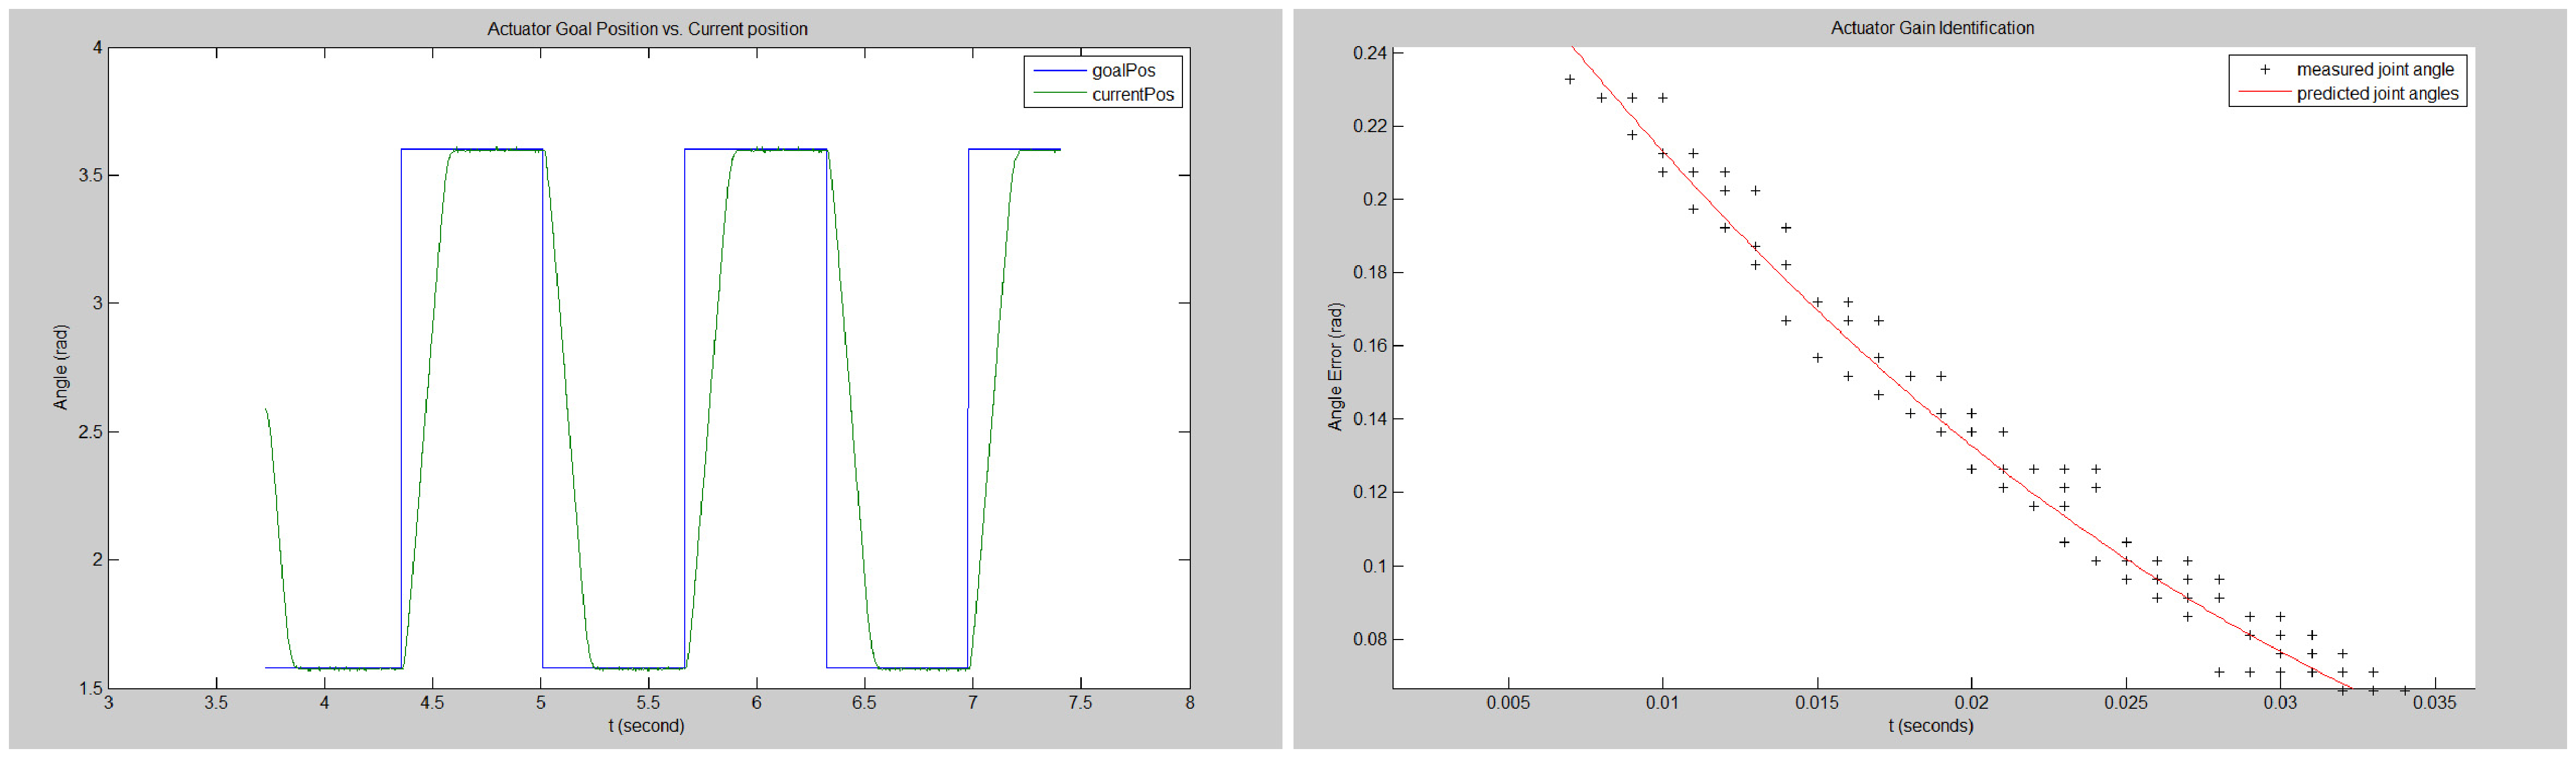
\includegraphics[width=0.5\textwidth]{figures/actuatorId}
  \caption{Actuator Identification. Left: the time series of input desired joint angle and the measured joint angle for an AX-18 servo. Right: the time series of actual error of joint angle and the predicted error using the identified actuator gains.  }
  \label{fig:actuatorId}
\end{figure}

Given $q(t)$ and $\bar{q}(t)$, we can apply regression to estimate the actuator gains. From eq. (\ref{eqn:torqueErrorRelationSimple}), we have
\begin{equation}
I\ddot{q}=-k_p(q-\bar{q}) - k_d\dot{q} - k_c\sgn(\dot{q})
\end{equation}
where $I$ is the moment of inertia of the foot with respect to the rotating axis. The above equation is derived by plugging into $\tau = I\ddot{q}+\dot{I}\dot{q}$ and the fact that $\dot{I}\dot{q}=0$ because the foot is a rigid body that rotates along a fixed axis. Ideally, $\ddot{q}$ and $\dot{q}$ can be computed using finite difference. However, the measurement of $q(t)$ is too noisy and finite difference would greatly magnify the noise. To solve this problem, we first smooth $q(t)$ by performing a 4th-order polynomial regression:
\begin{equation}
  \min_{a,b,c,d,e}\int ||q(t)-(at^4+bt^3+ct^2+dt+e)||^2\mathrm{d}t
  \label{eqn:Deltaq}
\end{equation}
where $a,b,c,d,e$ are the polynomial coefficients. This regression gives us a smooth analytical expression of $q(t)$. We then compute $\ddot{q}$ and $\dot{q}$ by differentiate this polynomial analytically:
\begin{align}
\label{eqn:Deltaqdot}  \dot{q}(t)&=4at^3+3bt^2+2ct+d\\
\label{eqn:Deltaqddot}  \ddot{q}(t)&=12at^2+6bt+2c
\end{align}

Combining eq. (\ref{eqn:Deltaq}), (\ref{eqn:Deltaqdot}) and (\ref{eqn:Deltaqddot}), we can perform another regression to compute the actuator gains.
\begin{equation}
\min_{k_p, k_d, k_c}\int||I\ddot{q}(t)+k_p(q(t)-\bar{q}(t)) + k_d\dot{q}(t) + k_c\sgn(\dot{q}(t))||^2\mathrm{d}t
\end{equation}

Our experiments and computation show that the actuator gains are $k_p=9.272(N\cdot m/rad)$, $k_d=0.3069(N\cdot m\cdot s/rad)$, and $k_c=0.03(N\cdot m)$. To verify the correctness of these values, we plug them into the simulator and repeat the same experiment in the simulation. The black ``+'' in Figure~\ref{fig:actuatorId} Left shows the error samples $q-\bar{q}$ in a small segment of time collected in the robot experiment. The red curve in Figure \ref{fig:actuatorId} Right is the error over time predicted in our simulation. They agree well.



\section{Controller Optimization}
\ignorethis{
\karen{If the goal is to create robust controllers, can we later use the calibrated simulation parameters to create a feedback controller (\eg using inverted pendulum model) via simulator?}
\jie{I hope so but I do not know. Since our experiments only cover open-loop control, it might not be necessary to speculate whether our system will work on feedback controller in the paper. But I still mention that extending the current system to feedback controllers is one of the future wok.}
\karen{I agree that this should be considered as future work. I belive that matching simulation and reality will be much more difficult for a feedback controller. I think of our algorithm as to match stability region of simulation with that of hardware. For open-loop controller, we need to match two points, but for feedback controller we need to match two manifolds.}}

Given the physical simulation, we can design controllers to enable the robot to achieve various locomotion tasks in the simulated environment. The four tasks that we use to test our system are rising from a sitting, leaning or kneeling position and flipping towards a handstand position (Figure \ref{fig:sit2Stand}, \ref{fig:lean2Stand}, \ref{fig:kneel2Stand} and \ref{fig:stand2Hand}). For each task, the joint configuration of the initial pose and the final pose are provided by the user. The goal of controller optimization is to find a sequence of control signals $\bar{\mathbf{q}}(t)$ so that the robot can move from the initial to the final pose without losing balance. We purposefully choose to use only open-loop controllers\footnote{The internal feedback loop in the actuators still exist but we do not alter this feedback loop in our controller design.} in this work, which means that the control signal $\bar{\mathbf{q}}(t)$ is a function of time $t$ and does not depend on the states of the robot. Using only the open-loop controller can better evaluate our system, especially simulation calibration, because the accuracy of the simulation becomes more critical if feedback control is not allowed.

We first formulate a trajectory optimization problem for each task.
\begin{align}
 \label{eqn:obj}&\max_{\bar{\mathbf{q}}(t),T} V_{ctrl}(\mathbf{x}(\bar{\mathbf{q}}(t)))\\
\nonumber  \mathrm{subject\;} &\mathrm{to} \\
\label{eqn:dyn1} & \mathbf{M}(\mathbf{x})\mathbf{\ddot{x}}+\mathbf{C}(\mathbf{x},\mathbf{\dot{x}}) =\boldsymbol{\tau}(\mathbf{q}, \dot{\mathbf{q}}, \bar{\mathbf{q}}) + \mathbf{J}^T\mathbf{f}\\
\label{eqn:boundary1}&\bar{\mathbf{x}}(0) = \mathbf{x}_0\\
\label{eqn:boundary2}&\bar{\mathbf{q}}(t) = \mathbf{q}_T, \text{if } t \geq T
\end{align}

\ignorethis{\karen{At this point, it is not clear how we get \vc{q} and \vc{f} in the optimization.}
\jie{Let's wait for Byron and see his opinion on this.}}
This optimization searches for the duration $T$ of the entire motion and the trajectory of the desired joint configuration $\bar{\mathbf{q}}(t)$ to maximize a task-related fitness function $V_{ctrl}$, and subject to physical constraints (eq.(\ref{eqn:dyn1})) and boundary conditions (eq.(\ref{eqn:boundary1}) and (\ref{eqn:boundary2})). $\mathbf{x}_0$ is the initial condition, and $\mathbf{q}_T$ is the final pose. Note that although we can specify the full state in the initial condition, we can only specify the desired joint angles for the final pose because the global translation and rotation are determined by the physical simulation.

We parameterize the desired trajectory $\bar{\mathbf{q}}(t)$ to reduce the dimension of the optimization problem. Although there are many ways that we can parameterize the control space, designing the most effective control parametrization is not the focus of this work. In this work, we choose a simple parametrization that use a sparse set of keyframes $\bar{\mathbf{q}}_1, \bar{\mathbf{q}}_2, ..., \bar{\mathbf{q}}_n$. Between the keyframes, we linearly interpolate the poses from two adjacent keyframes. With this simplification, the \emph{control parameters} that we need to optimize reduce to only a few keyframes and the time intervals between adjacent keyframes.

\ignorethis{
\karen{Why do we have to assume no inter-body collision? There are many other possible ways that the desired trajectoires achieve the objective in an undesired way (\eg jump of the ground), do we also need to assume that those situations won't happen? More fundamental question: how can we make any of these assumptions while our optimizer doesn't know about these assumptions?}
\jie{I removed the first few sentences that confuse you. Actually we do not assume anything. If the robot jumps off the ground in the simulation, we do not do anything to prevent that. You can see this from the video of stand-to-handstand. Before simulation calibration, the optimal controller indeed jumps in the simulation. But after calibration, the optimal controller does not jump in the simulation, which matches the real world performance. In term of self-collision, it did not happen because we chose a reasonable range of joint angles to search in CMA.}
\karen{That sounds fine.}
}

The criterion of success for all the tasks is whether the robot remains upright at the end of its motion. We use the following fitness function to reward controllers that keep balance throughout the entire motion.


\begin{equation}
  V_{ctrl}(\mathbf{x}(\bar{\mathbf{q}}(t)))=\int_0^{T+1} \frac{1}{\alpha(\bar{\mathbf{q}}(t))+\epsilon}\mathrm{d}t
  \label{eqn:controllerObj}
\end{equation}
where $\alpha$ is the angle between the up direction in the local frame of the robot's torso and the up direction in the global frame $(0,0,1)$. It measures how far the robot is from losing its balance. $\epsilon$ is a small positive number to prevent the denominator from being zero. We choose $\epsilon=0.1$ in all our tasks. Note that the upper limit of the integration is $T+1$. The extra one second is to wait for the robot to settle down. We use the time horizon $T+1$ because it is still possible that the robot can fall during the settling down phase and our fitness function will penalize this situation.

During locomotion, discrete contact events can happen frequently. They impose additional challenges for the continuous optimization algorithms that rely on gradient information. To overcome this challenge, we choose to use CMA to optimize the control parameters. CMA is a sample-based stochastic optimization algorithm, which has a solid theoretical foundation \cite{akimoto:2010,glasmachers:2010}. It does not need gradient information and can explore multiple local minima. This makes it ideal to optimize controllers for locomotion tasks. For the completeness of the paper, we will briefly describe the CMA algorithm here. Please refer to the original paper \cite{Hansen:2009} for more details. At each iteration, a population of CMA samples are drawn from an underlying Gaussian distribution. In our case, a CMA sample is a candidate controller. Each CMA sample is then simulated and evaluated using eq.(\ref{eqn:controllerObj}). The samples with lower fitness values are discarded. The underlying Gaussian distribution is updated according to the remaining good samples. With more iterations, the distribution gradually converges to a better region of the control space. After a maximum number of iterations, we choose the best CMA sample as the output of the controller optimization subsystem.

\section{Simulation Calibration}
\ignorethis{\karen{Need to motivate why we pick these simulation parameters.}}
Although the optimal controllers $\bar{\mathbf{q}}(t)$ can work effectively in the simulation, they may fail to achieve the tasks in the real world. One cause of this failure is the erroneous parameter settings in the physical simulation, such as the mass, the moment of inertia, the COM of each body segment, and the gains of the actuators. Usually, simulation parameters are set according to the specification of the robot. However, we find that many of these specifications are inaccurate. For example, there is about 40\% of error in the total mass of our robot between the open-source CAD file and our own measurement. Instead of trusting these parameters, we decide to adjust them in simulation calibration. We formulate an optimization that searches for the simulation parameters $\boldsymbol{\theta}$ to minimize the discrepancy $E_{cali}$ between the simulated results and the robot performance in the real environment.

\begin{equation}
 \min_{\boldsymbol{\theta}} E_{cali}
\label{eqn:calibration}
\end{equation}

Although there are dozens of simulation parameters $\boldsymbol{\theta}$ that we could calibrate, we choose to focus on the gains of the actuators and the COM of each body segment. We believe that they are the most relevant parameters to our tasks. Our tasks involve changing postures and maintaining balance. We decide to calibrate only actuator gains and COM because the actuator gains are critical to posture change and the COM is vital to balance.

$E_{cali}$ is defined as the difference between the state trajectories in the simulation and those collected in the real robot experiments when the same controller is used in both scenarios:

\begin{equation}
  E_{cali}=\frac{1}{n}\sum_{i=1}^{n}\int_{0}^{T+1}||\tilde{\mathbf{x}}_i(t)-\mathbf{x}_i(t)||_{\mathbf{W}}^2\mathrm{d}t
  \label{eqn:calibrationObj}
\end{equation}
Recall that our entire algorithm is an iterative process. At the $n$th iteration, the optimal controller $\bar{\mathbf{q}}_n(t)$ produces the state trajectory $\mathbf{x}_n(t)$ in the simulation and $\tilde{\mathbf{x}}_n(t)$ on the real robot\footnote{we use the average of the multiple trajectories as $\tilde{\mathbf{x}}_n(t)$ in the robot experiment because even with the same controller, we can get slightly different trajectories due to the varied initial conditions, the noise from the sensor, from the actuator and from the environment.}. $E_{cali}$ is measured using all $n$ optimal controllers $\{\bar{\mathbf{q}}_i(t)\}_{i=1,...,n}$ and their associated state trajectories $\{\bar{\mathbf{x}}_i(t)\}_{i=1,...,n}$ from the current and the previous iterations. $\mathbf{W}$ is a weight matrix, which encapsulates the relative importance of each joint.

Due to the presence of contact changes in the locomotion task and the complex interplay between the simulation results and the simulation parameters, the optimization (\ref{eqn:calibration}) is challenging using traditional continuous optimization algorithms. Similar to controller optimization, we choose to use CMA as the optimization solver. In this case, each CMA sample is a candidate set of simulation parameters $\boldsymbol{\theta}$. To evaluate each CMA sample, we set the parameters $\boldsymbol{\theta}$ in the physical simulator, execute the controllers $\{\bar{\mathbf{q}}_i(t)\}_{i=1,...,n}$ to simulate the robot motions $\{\mathbf{x}_i(t)\}_{i=1,...,n}$, and then evaluate the objective function eq. (\ref{eqn:calibrationObj}).


\section{Results}

\begin{figure*}[!t]
  \centering
  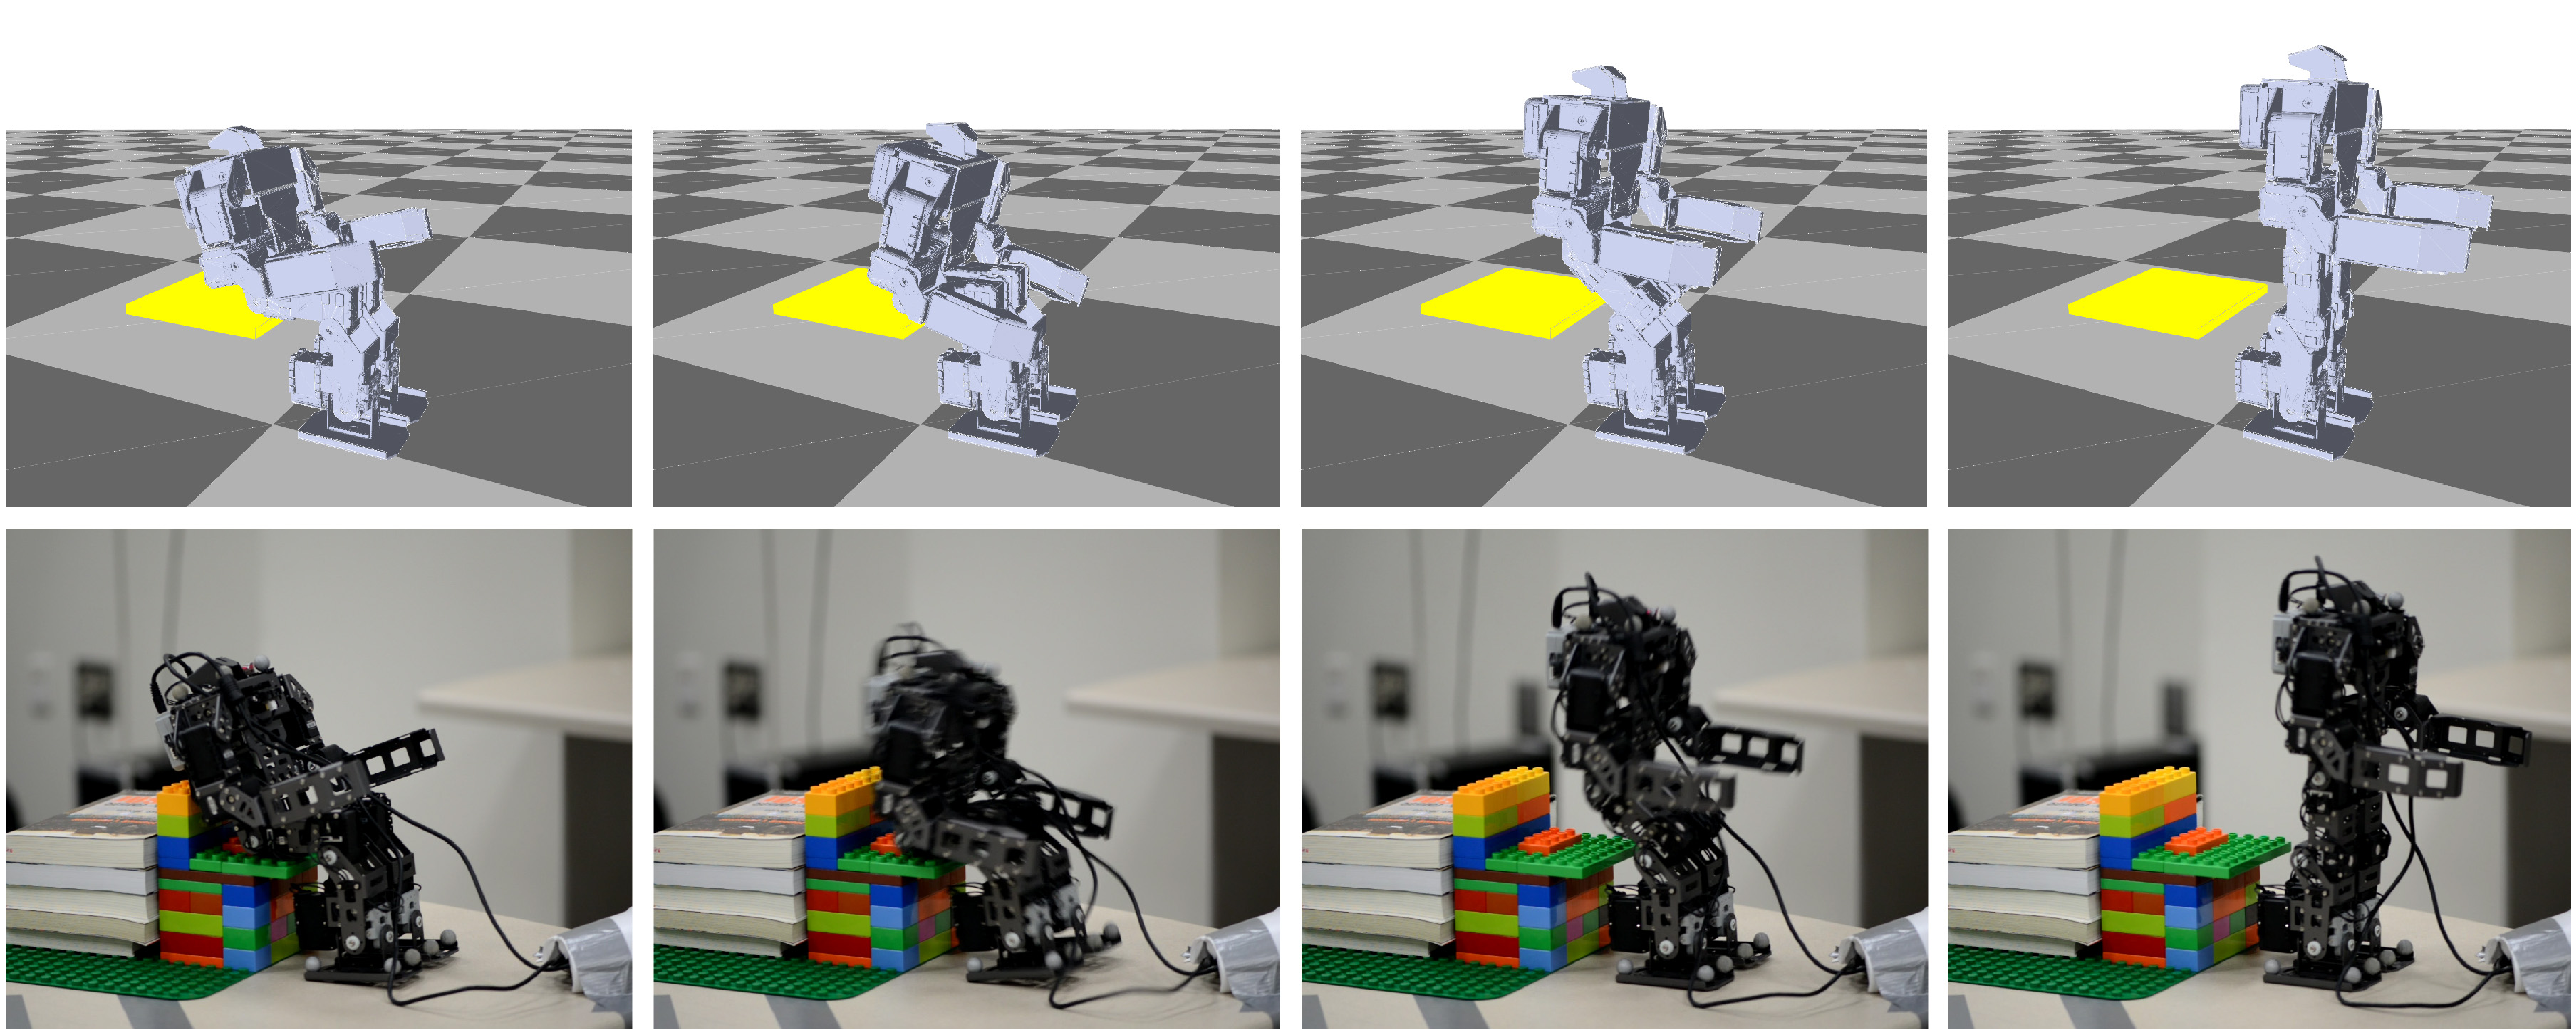
\includegraphics[width=\textwidth]{figures/sit2Stand}
  \caption{The results of the sit-to-stand task in the simulation and on the real robot.}
  \label{fig:sit2Stand}
\end{figure*}

In this section we present the results of our system. We use four locomotion tasks to evaluate our system: The robot rises from a leaning, sitting or kneeling position and flipping to a handstand pose. Please watch the accompanying video for the robot performance in the simulation and in the real world.

\subsection{Experiment Setup}

We use BIOLOID GP as our robot platform. BIOLOID GP is a humanoid robot that consists of 18 degrees of freedom that are powered by Dynamixel AX-12/AX-18 servos. The communication between the PC and the robot is through a serial port. To control the robot, a master program on the PC writes the desired pose $\bar{\mathbf{q}}$ to the serial port that is connected to the robot. A slave program that runs on the robot's onboard microprocessor listens to this port and sends the desired joint angle to each actuator. At the same time, the robot performance data $\tilde{\mathbf{x}}$ is measured and sent back to the computer. We use onboard rotary encoders to measure joint angles and a VICON motion capture system to measure the global position and orientation of the robot's torso. The average latency of the whole control loop on our robot is 16ms. It is measured by a timer in our program between the time when the master program starts sending the actuator commands to the robot and when it finishes reading the sensor measurements from the robot.

\subsection{Implementation Details}

Our system is implemented in C++ and runs on a laptop with a 2.6GHz quad-core CPU and 16GB of memory. We use DART to simulate the physics of the robot and its surrounding environments. In our work, we initialize the simulation parameters as follows. We set the physical properties of each body segment, including the mass, the moment of inertia and the COM according to the CAD files. We set the actuator gains based on the measurement from experiments (Section \ref{sec:motorDynamics}). We leave all other parameters as default values in DART. Although these parameters are not accurate, they serve as a good initial guess. We use 1ms as the time step in physical simulation. We recompute the control signal every 16 time steps in the simulation to mimic the actual control latency on the robot.

We find that all four tasks can be achieved with symmetric lower body motions. This observation enables us to reduce the dimensionality of the control space. In controller optimization, we halve the size of the optimization problem by exploiting this symmetry of the motion. We constrain that the joint motions on the left bodies mirror those on the right bodies. In addition, we also constrain our optimization to the lower body motions.

During simulation calibration, we search for the simulation parameters within a bounded range centered at their initial settings. Although there are dozens of simulation parameters that can be calibrated at this stage, we choose to focus on the COM of each body segment and the actuator gains since they are the most relevant parameters to the success of our locomotion tasks. In all the experiments, we choose the weights $\mathbf{W}$ in the objective function (eq. (\ref{eqn:calibrationObj})) such that $E_{cali}$ measures the difference of the global orientations of the root body between in the simulation and in the real world. For each simulation calibration, we collect three episodes of robot data by running the same controller three times to average out the noise and initial condition perturbations. Each episode is approximately two seconds.

The parameter settings of CMA for both controller optimization and simulation calibration are the same. We use 32 CMA samples per iteration and at most 50 iterations. We distribute the computation across all four cores of the CPU. It takes less than 15 minutes to find an optimal solution in controller optimization or simulation calibration.

\begin{figure}[!t]
  \centering
  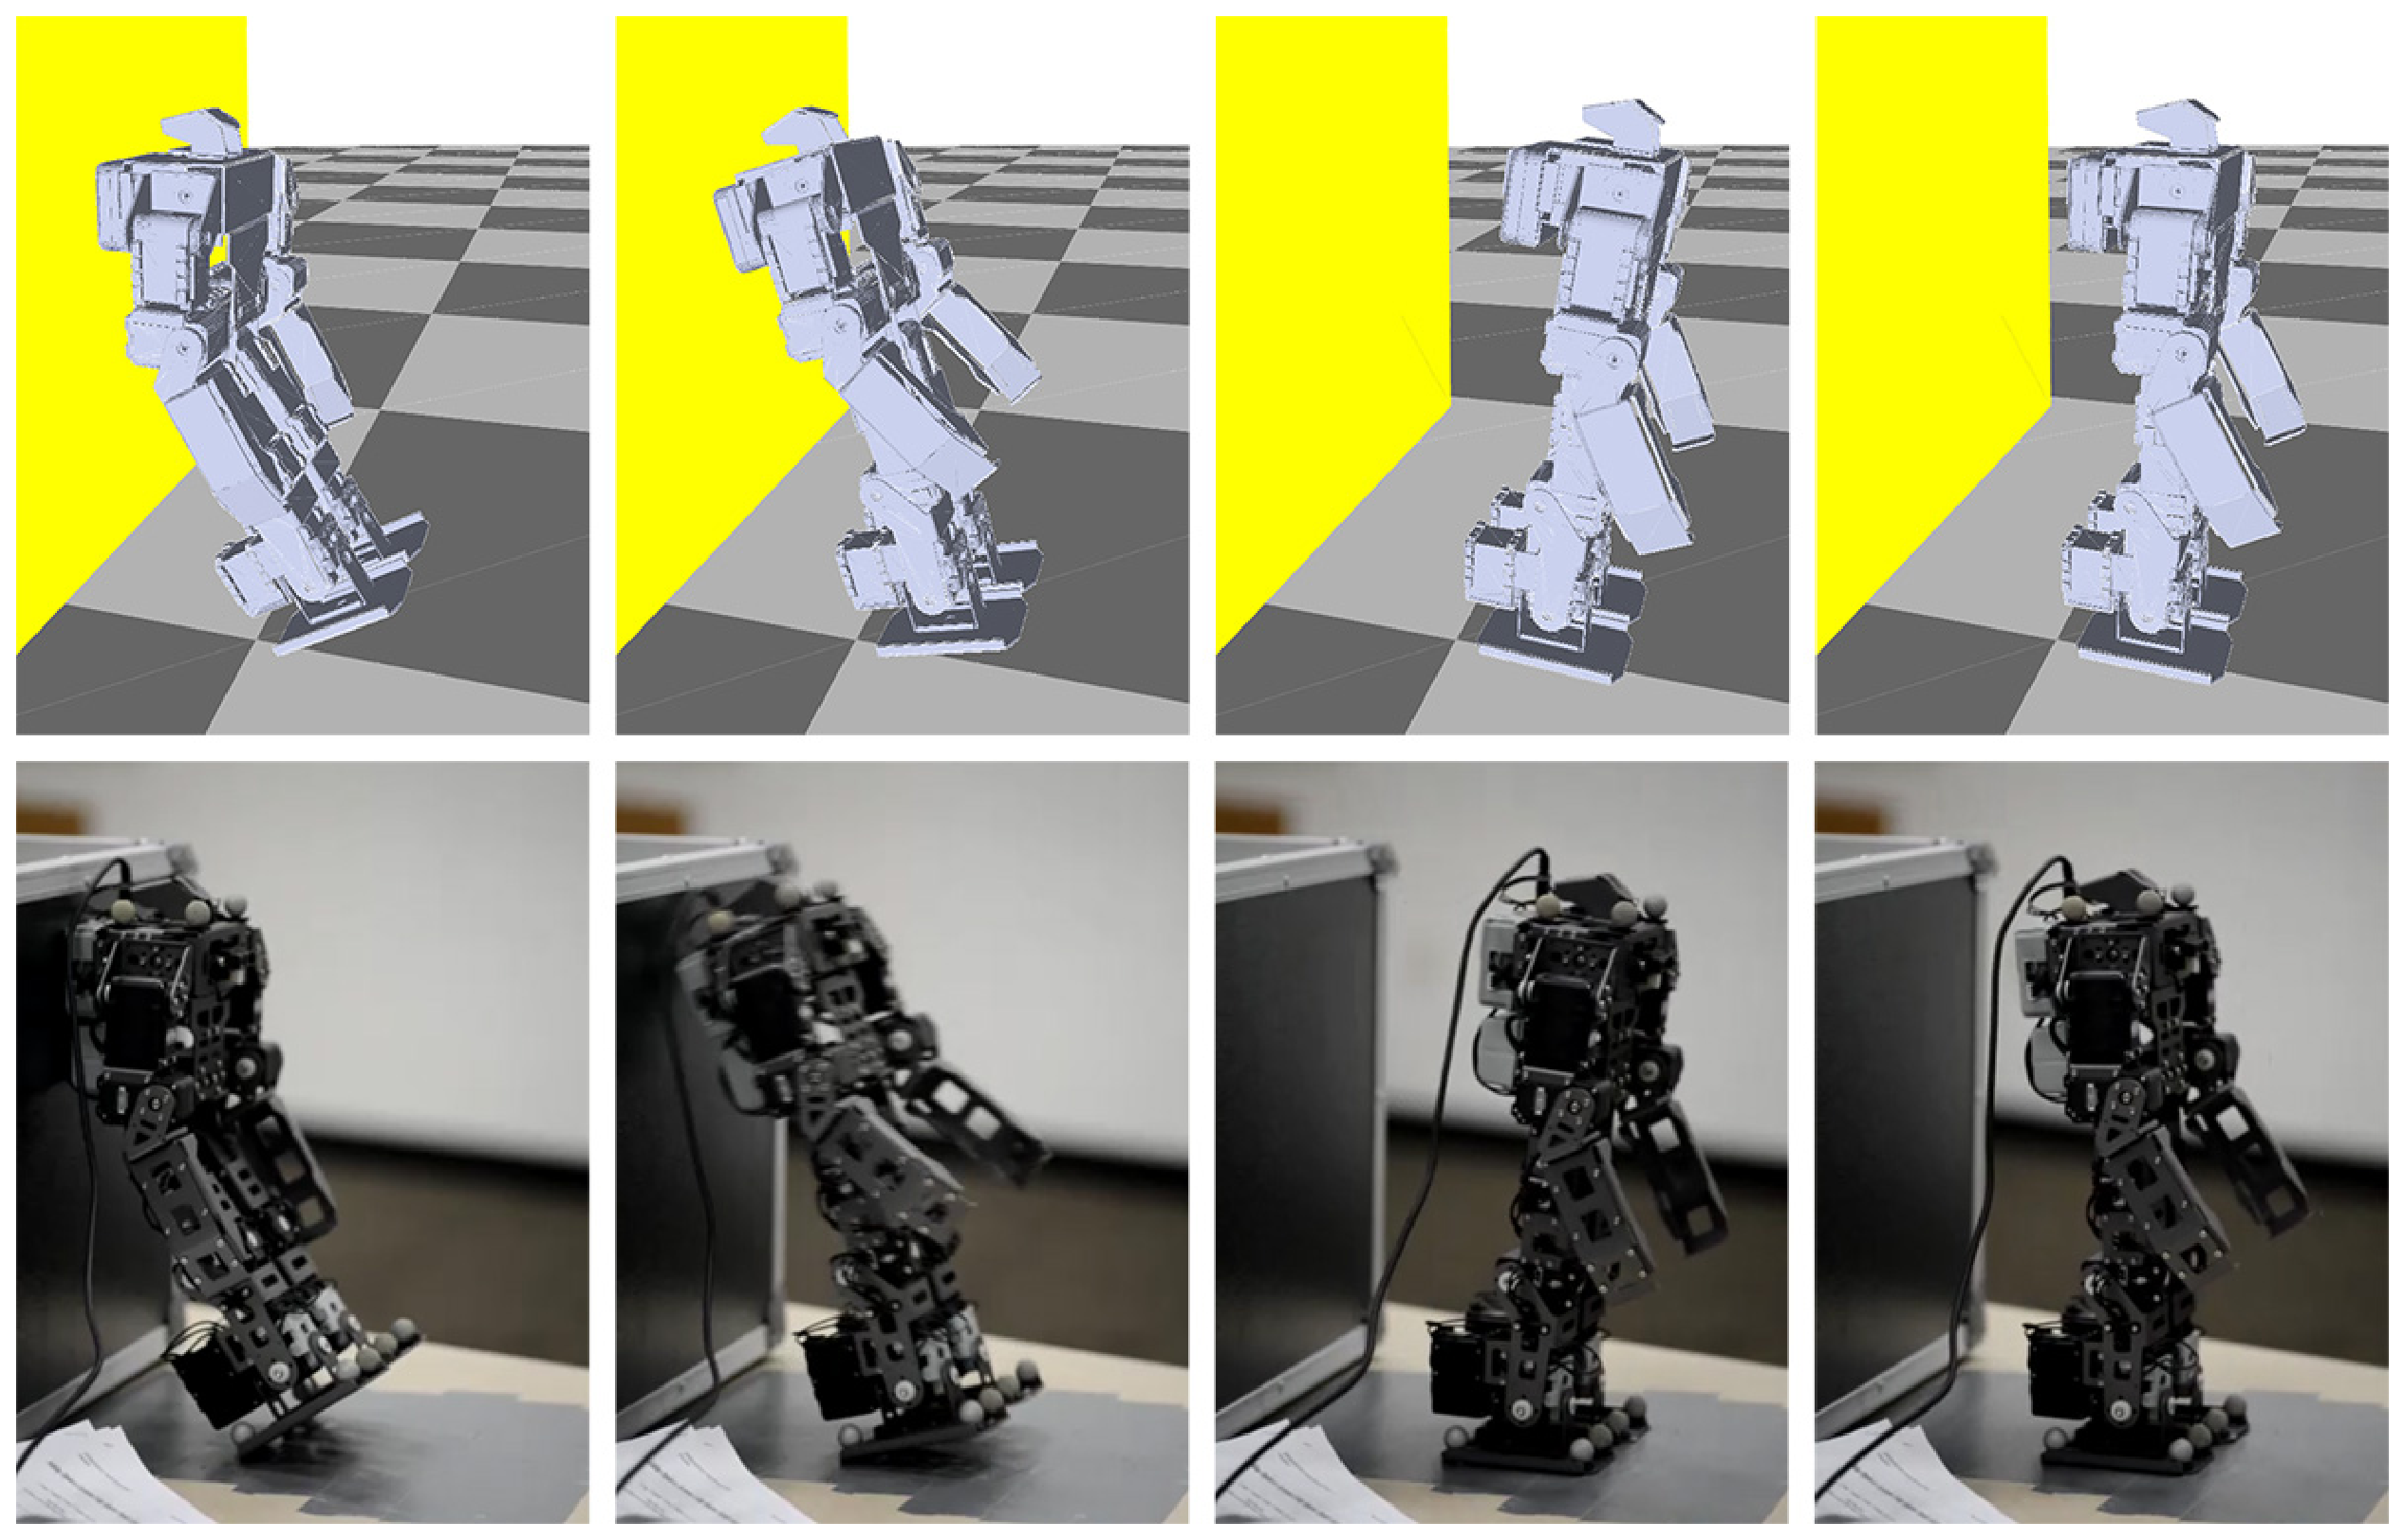
\includegraphics[width=0.5\textwidth]{figures/lean2Stand}
  \caption{The results of the lean-to-stand task in the simulation and on the real robot.}
  \label{fig:lean2Stand}
\end{figure}

\subsection{Rising from a Sitting Position}

The first task that we have tested is to rise from a sitting pose to a standing pose (Figure \ref{fig:sit2Stand}). The initial and the final poses $q_0$ and $q_T$ are shown in the leftmost and rightmost images in Figure \ref{fig:sit2Stand}. The controller optimization needs to search for an additional inbetween keyframe $q_1$, as well as the two time intervals $t_1$ and $t_2$ between these three keyframes. 

We intentionally choose the initial pose that the legs of the robot extend forward and the projection of the robot's COM in the vertical direction falls far behind the contact points of the feet. If the robot simply extends the hips and the knees to stand up, it will fall backwards. Despite this challenging setup, our system successfully finds a controller that enables the robot to stand up in the simulation. Figure \ref{fig:sit2Stand} shows that the robot first builds up a forward momentum by quickly leaning its upper body to the front. It then starts to extend the hips and the knees at the moment when the COM is approaching the boundary of the support polygon spanned by the feet. This effective standing-up strategy is found automatically by the controller optimization subsystem.

When applying this controller to the real robot, we are surprised to find that it works directly, without the need of simulation calibration. The robot stands up from a chair in the same way as its simulated counterpart does in the virtual world. This shows that the Reality Gap is not always a problem. In some tasks, the stability region of a controller is so large that it can make the discrepancy between the virtual and the real world less critical.

\subsection{Rising from a Leaning Position}

In this task, the robot needs to rise from leaning on the wall to a standing position (Figure \ref{fig:lean2Stand}). In the initial configuration, the hip joints are bent and they are straightened out in the final configuration while all other joints do not move. The initial and the final poses are the only two keyframes for this task.

\begin{figure}[!b]
  \centering
  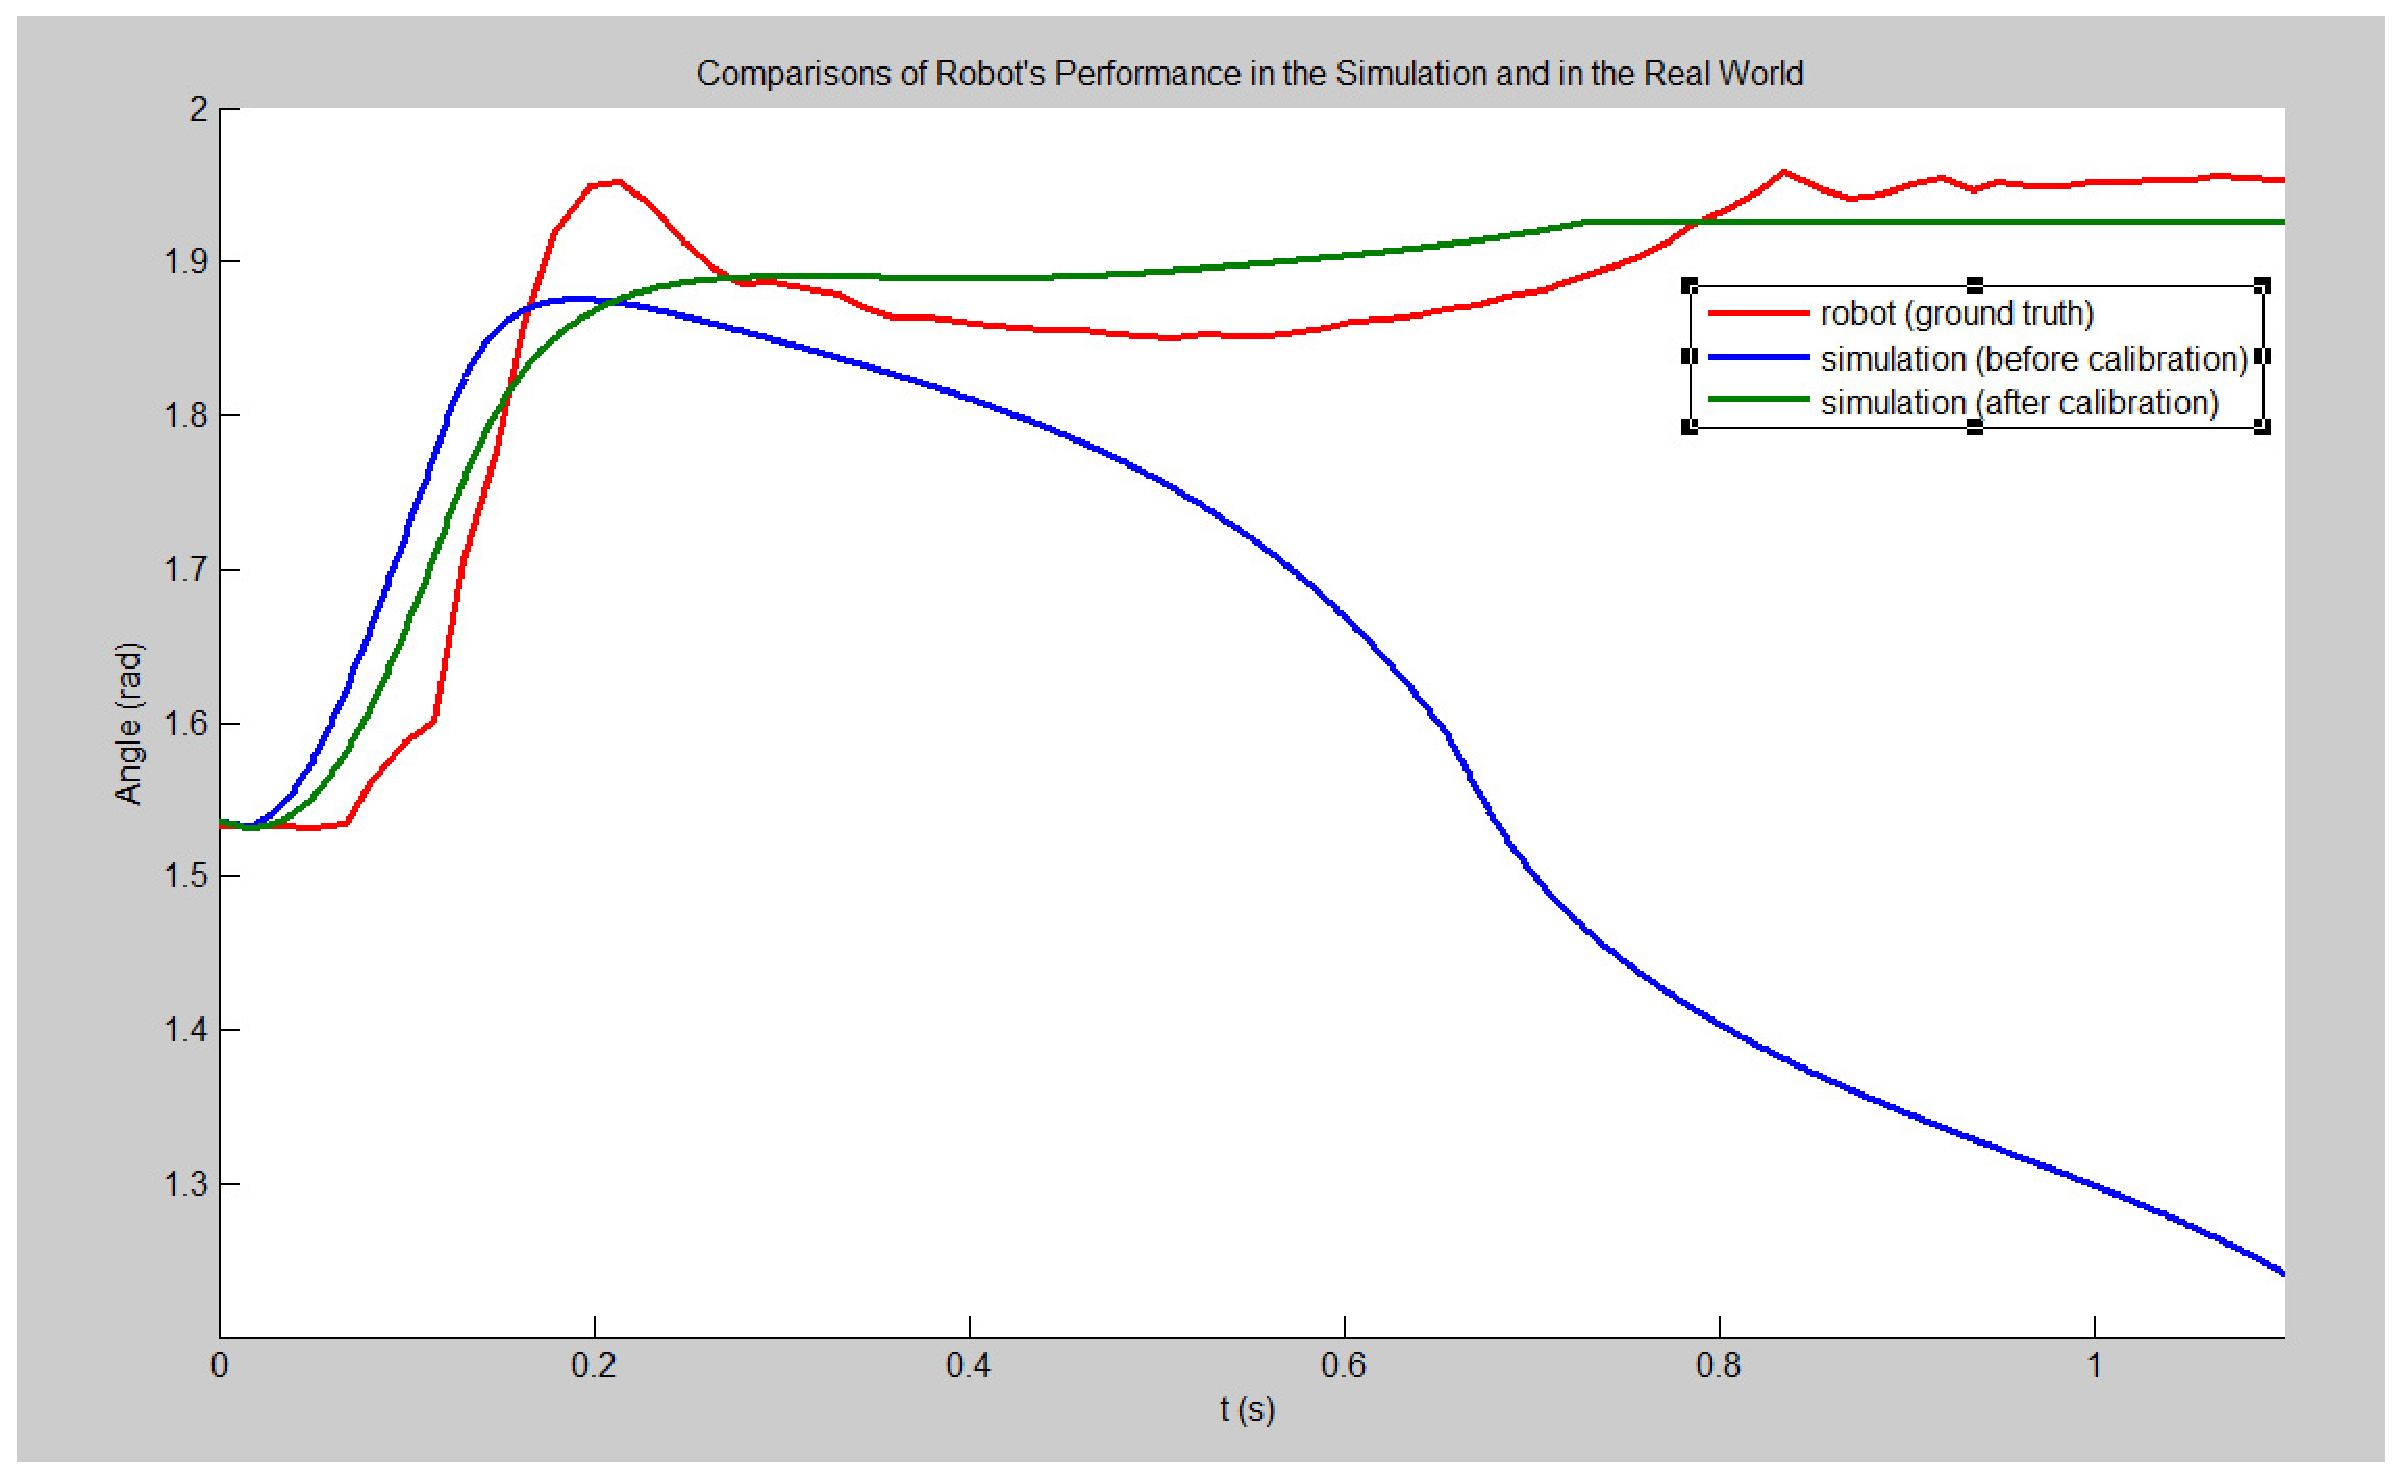
\includegraphics[width=0.4\textwidth]{figures/simRobotCompare}
  \caption{Comparisons of the robot's global orientation over time in the simulation (before/after calibration) and in the real environment.}
  \label{fig:simRobotCompare}
\end{figure}


The goal of controller optimization is to find an appropriate time interval $T$ between these two keyframes. If the time interval is too long, the robot moves slowly, and cannot accumulate enough momentum to rise. If this time interval is too short, the robot move abruptly, which will cause the upper body to bounce off the wall too quickly and fall forward. Without simulation calibration, the controller optimization cannot find a working controller for this task. The robot cannot rise when $T\leq 0.10s$ and overshoots when $T > 0.10s$. Nevertheless, we apply the controller with the highest fitness value $T=0.11s$ on the robot. In contrast to the simulation result, in which the simulated robot rises too quickly and falls forward, the robot in the real world actually cannot rise. Figure \ref{fig:simRobotCompare} compares the trajectories of the robot's global orientation in the simulation (blue curve) and in the real world (red curve). After one iteration of simulation calibration, the discrepancy is greatly reduced (Figure \ref{fig:simRobotCompare} green curve). We optimize the controller again in this calibrated simulator. This time, the optimal controller works both in the simulated and in the real world.

\begin{figure}[!b]
  \centering
  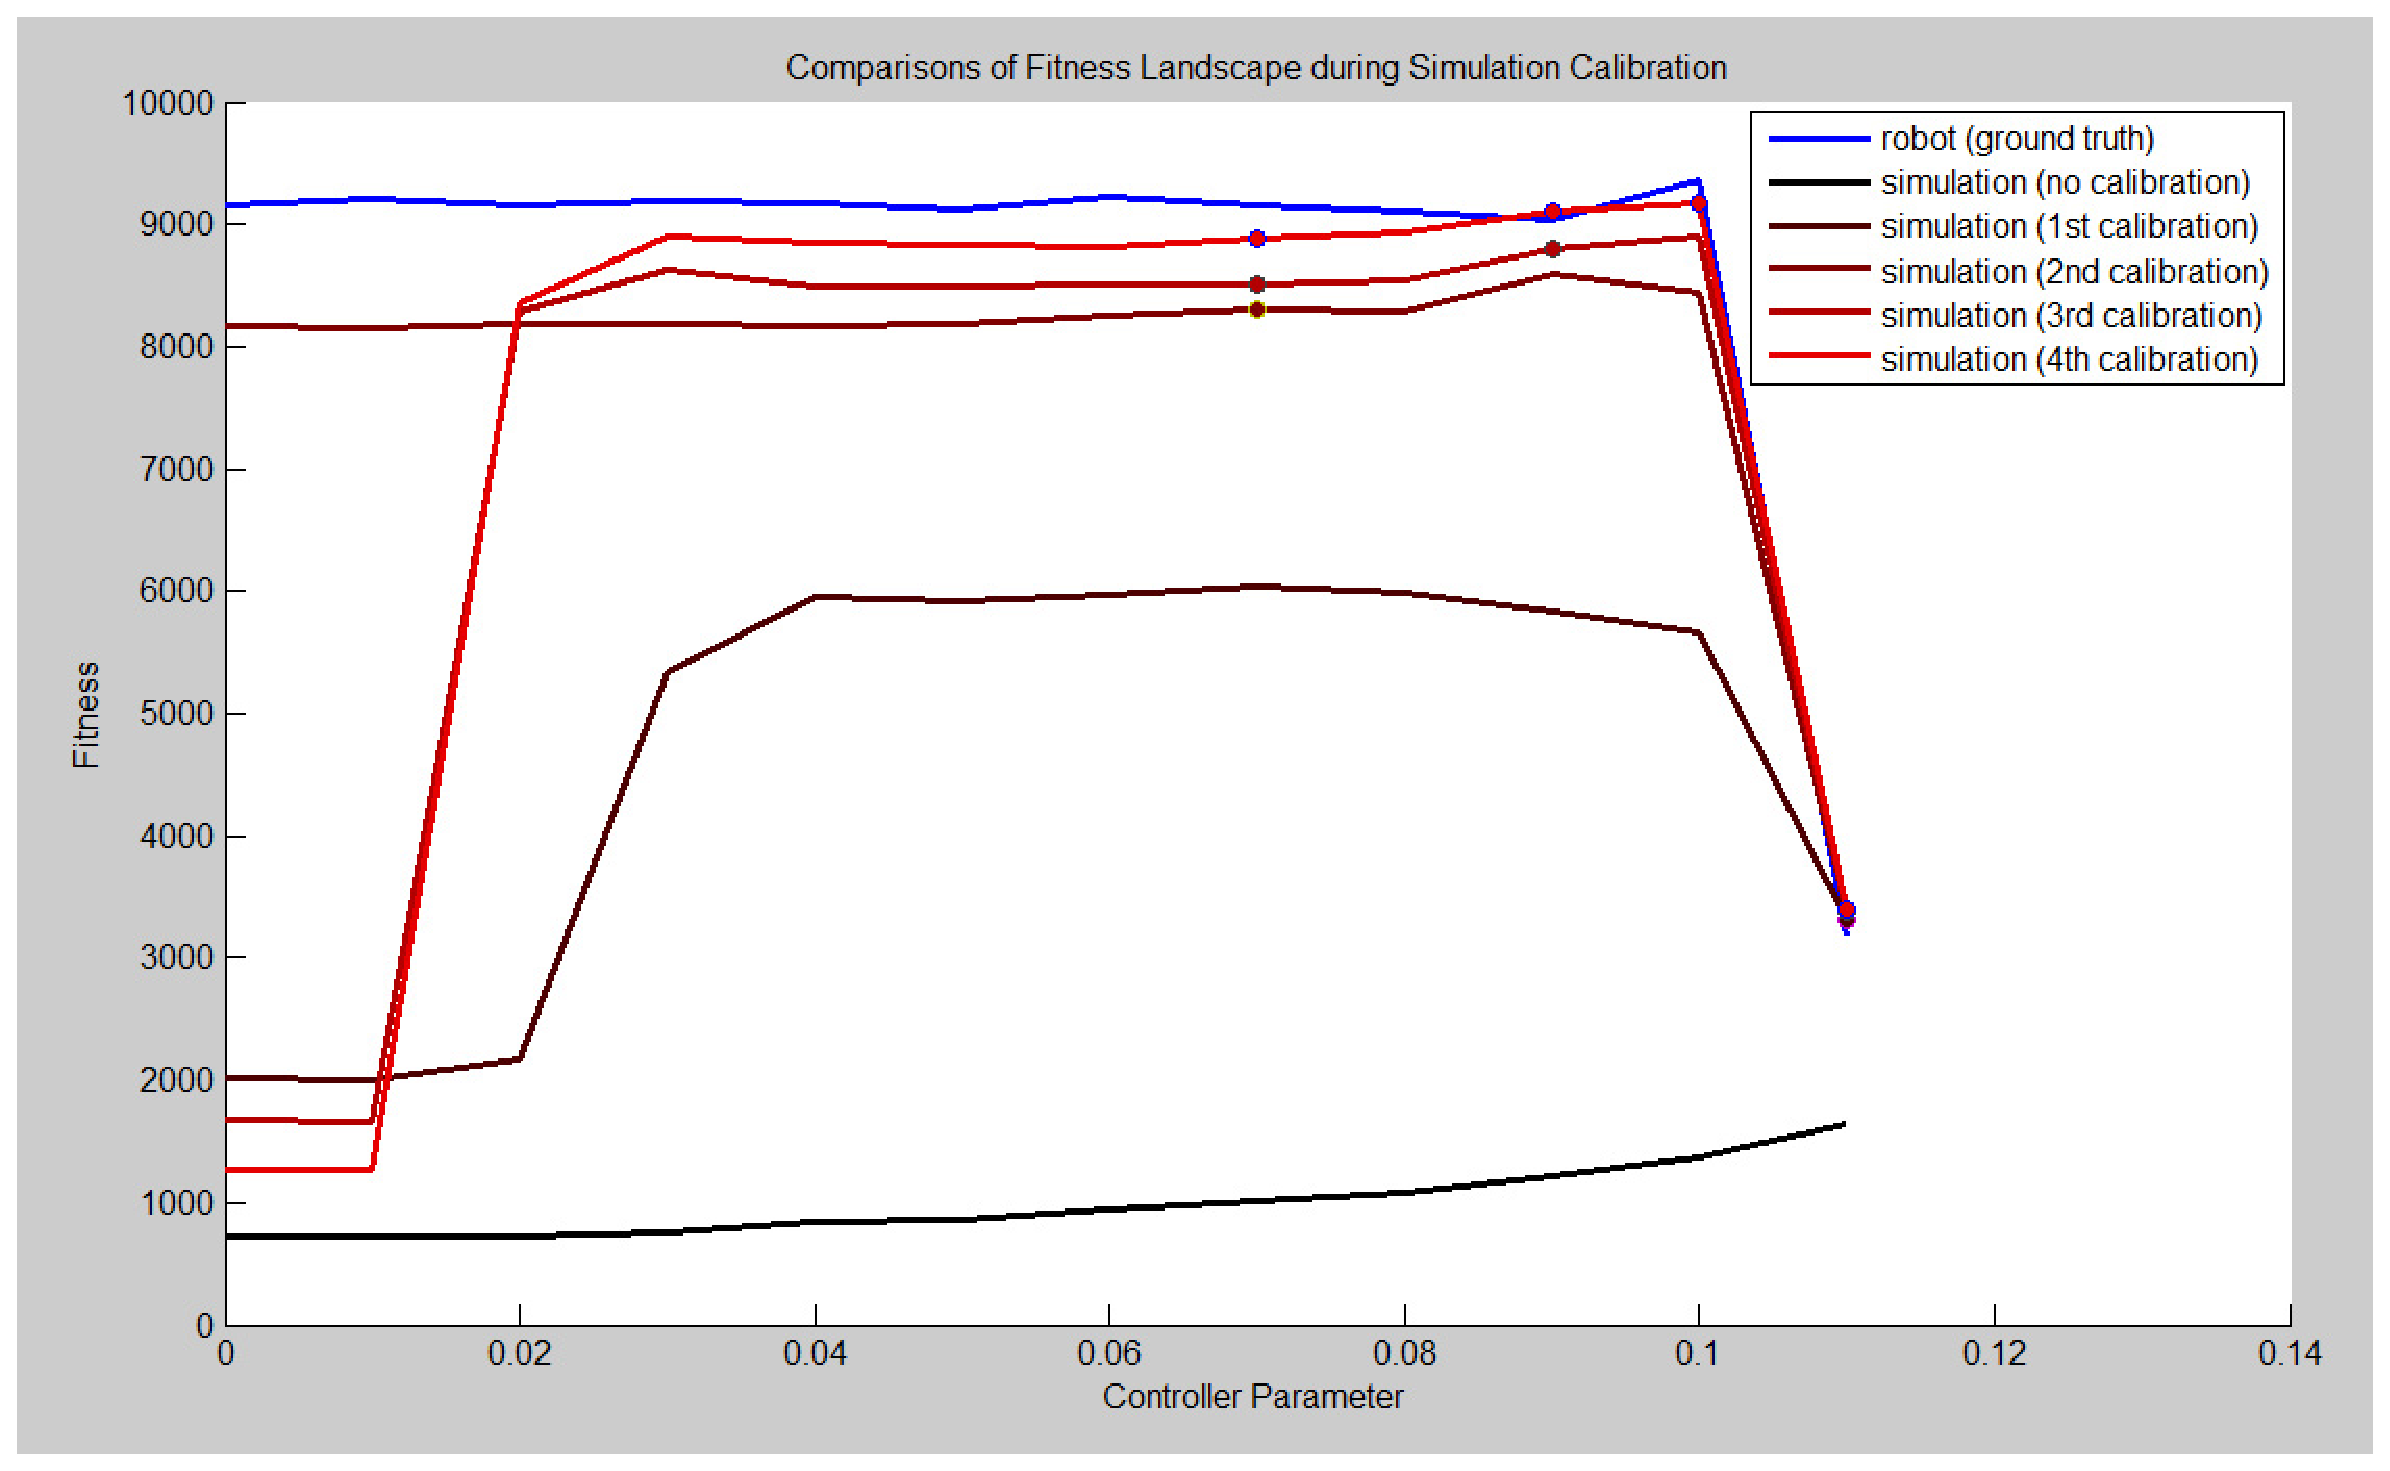
\includegraphics[width=0.4\textwidth]{figures/fitnessLandscape}
  \caption{Comparisons of the fitness landscape as more iterations of simulation calibration are performed.}
  \label{fig:fitnessLandscape}
\end{figure}

\begin{figure*}[!t]
  \centering
  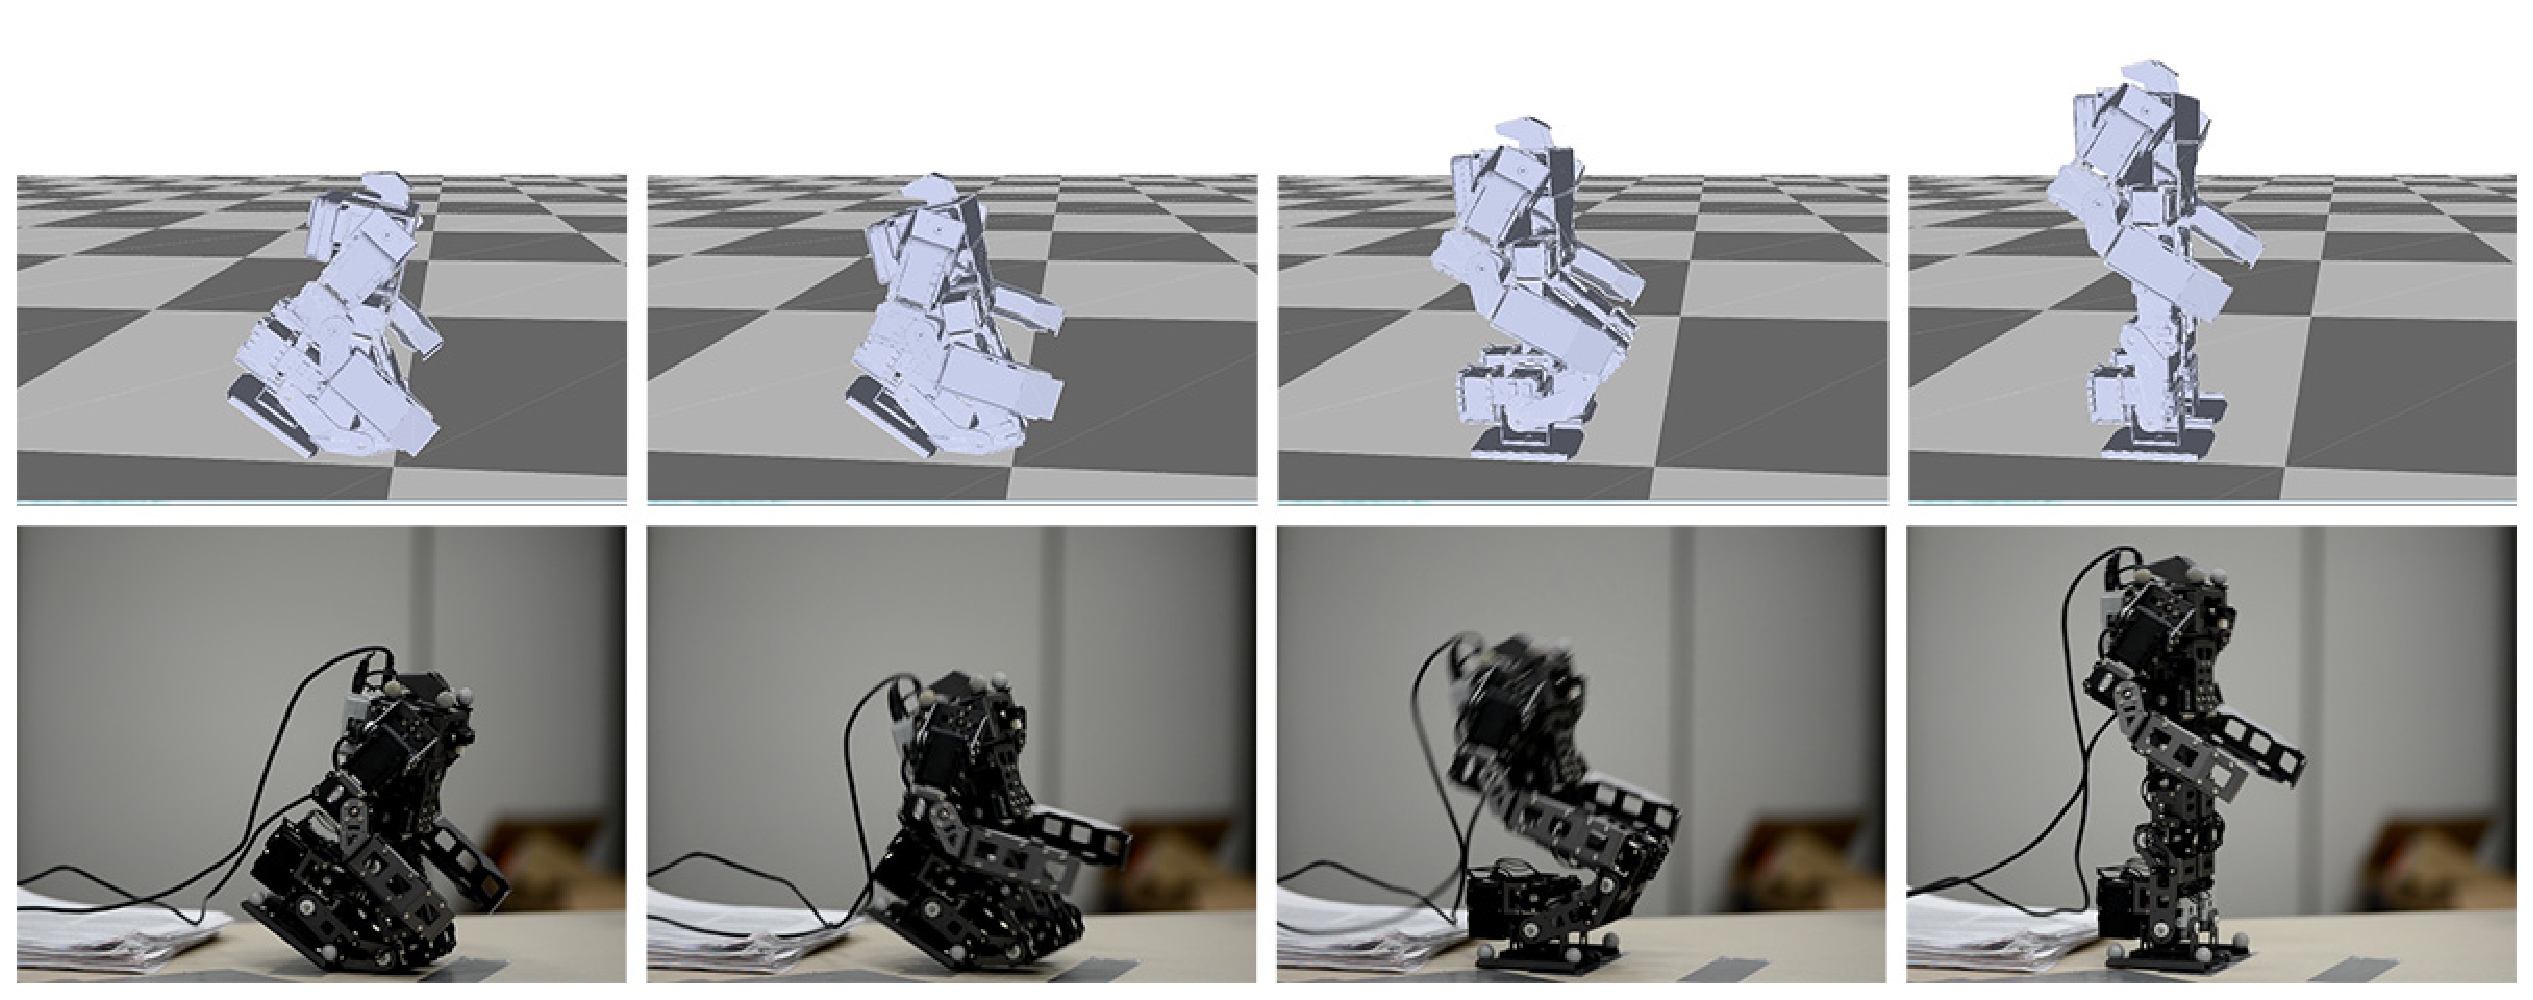
\includegraphics[width=\textwidth]{figures/kneel2Stand}
  \caption{The results of the kneel-to-stand task in the simulation and on the real robot.}
  \label{fig:kneel2Stand}
\end{figure*}

We successfully cross the Reality Gap with one iteration of simulation calibration, which uses only three episodes of robot experiments and totally 6 seconds of robot data. To better understand how the Reality Gap is gradually narrowed by simulation calibration over multiple iterations, we perform an additional evaluation. Figure \ref{fig:fitnessLandscape} shows how the fitness landscape in the simulation changes with different number of iterations of simulation calibration. The blue curve is the ground truth. It is evaluated on the real robot by varying the control parameter $T$ in the range of $[0, 0.11]$. The fitness value is calculated according to eq. (\ref{eqn:controllerObj}). The fitness landscape stays at a high value when $T\in[0, 0.1]$, which means that the real robot can successfully rise if the controller uses less than 0.1s to change the pose from the initial to the final configuration. In contrast, without simulation calibration, the fitness landscape (lowest black curve) stays at a low value for the entire control space. In other words, no controller exists that can make the robot stand up in the simulation. The gap between the blue and the black curves is analogue to the Reality Gap. One iteration of simulation calibration brings the fitness landscape in the simulation towards the ground truth. As more iterations are performed, the fitness landscape in the simulation (brown and red curves) gradually approaches the ground truth, and the Reality Gap is narrowed in this process. Note that a large discrepancy still exists in the region of the parameter space where $T<0.02s$. This is probably caused by two reasons. First, in the region of $T<0.02s$, the torque output of the servo is at its limit but the torque limit is not considered in simulation calibration. Second, the controllers and the data (the red circles in Figure \ref{fig:fitnessLandscape}) that we use in simulation calibration concentrate on the right half of the parameter space, which makes it difficult to generalize to a region where the data is scarce ($T<0.02$). However, this is beneficial in our applications because the computational resource is focused at the important regions near the successful controllers. This explains why our system can find a successful controller in the real word with minimal robot experiments.

\subsection{Rising from a Kneeling Position}

Figure \ref{fig:kneel2Stand} shows that the robot stands up from a kneeling pose. Between the user-specified initial and final poses, the controller consists of two additional keyframes. The optimization needs to search for these keyframes and the time intervals between adjacent keyframes. The controller optimized in the simulation demonstrates an agile getting-up motion: The robot first leans its upper-body backwards. As its COM is moving to the back, it quickly bends the hip, flexes its ankles and stands up. This entire motion resembles one of the most agile ways that we human get up from a kneeling position when we do not use our hands for additional support. Although this controller works perfectly in the simulation, the robot falls backward in the real world. After simulation calibration, the performance of the simulated robot comes closer to the real world scenario. Using the calibrated simulator, we optimize a new controller, with which the robot can successfully stand up from the kneeling position in the real world (Figure \ref{fig:kneel2Stand}).

\begin{figure*}[!t]
  \centering
  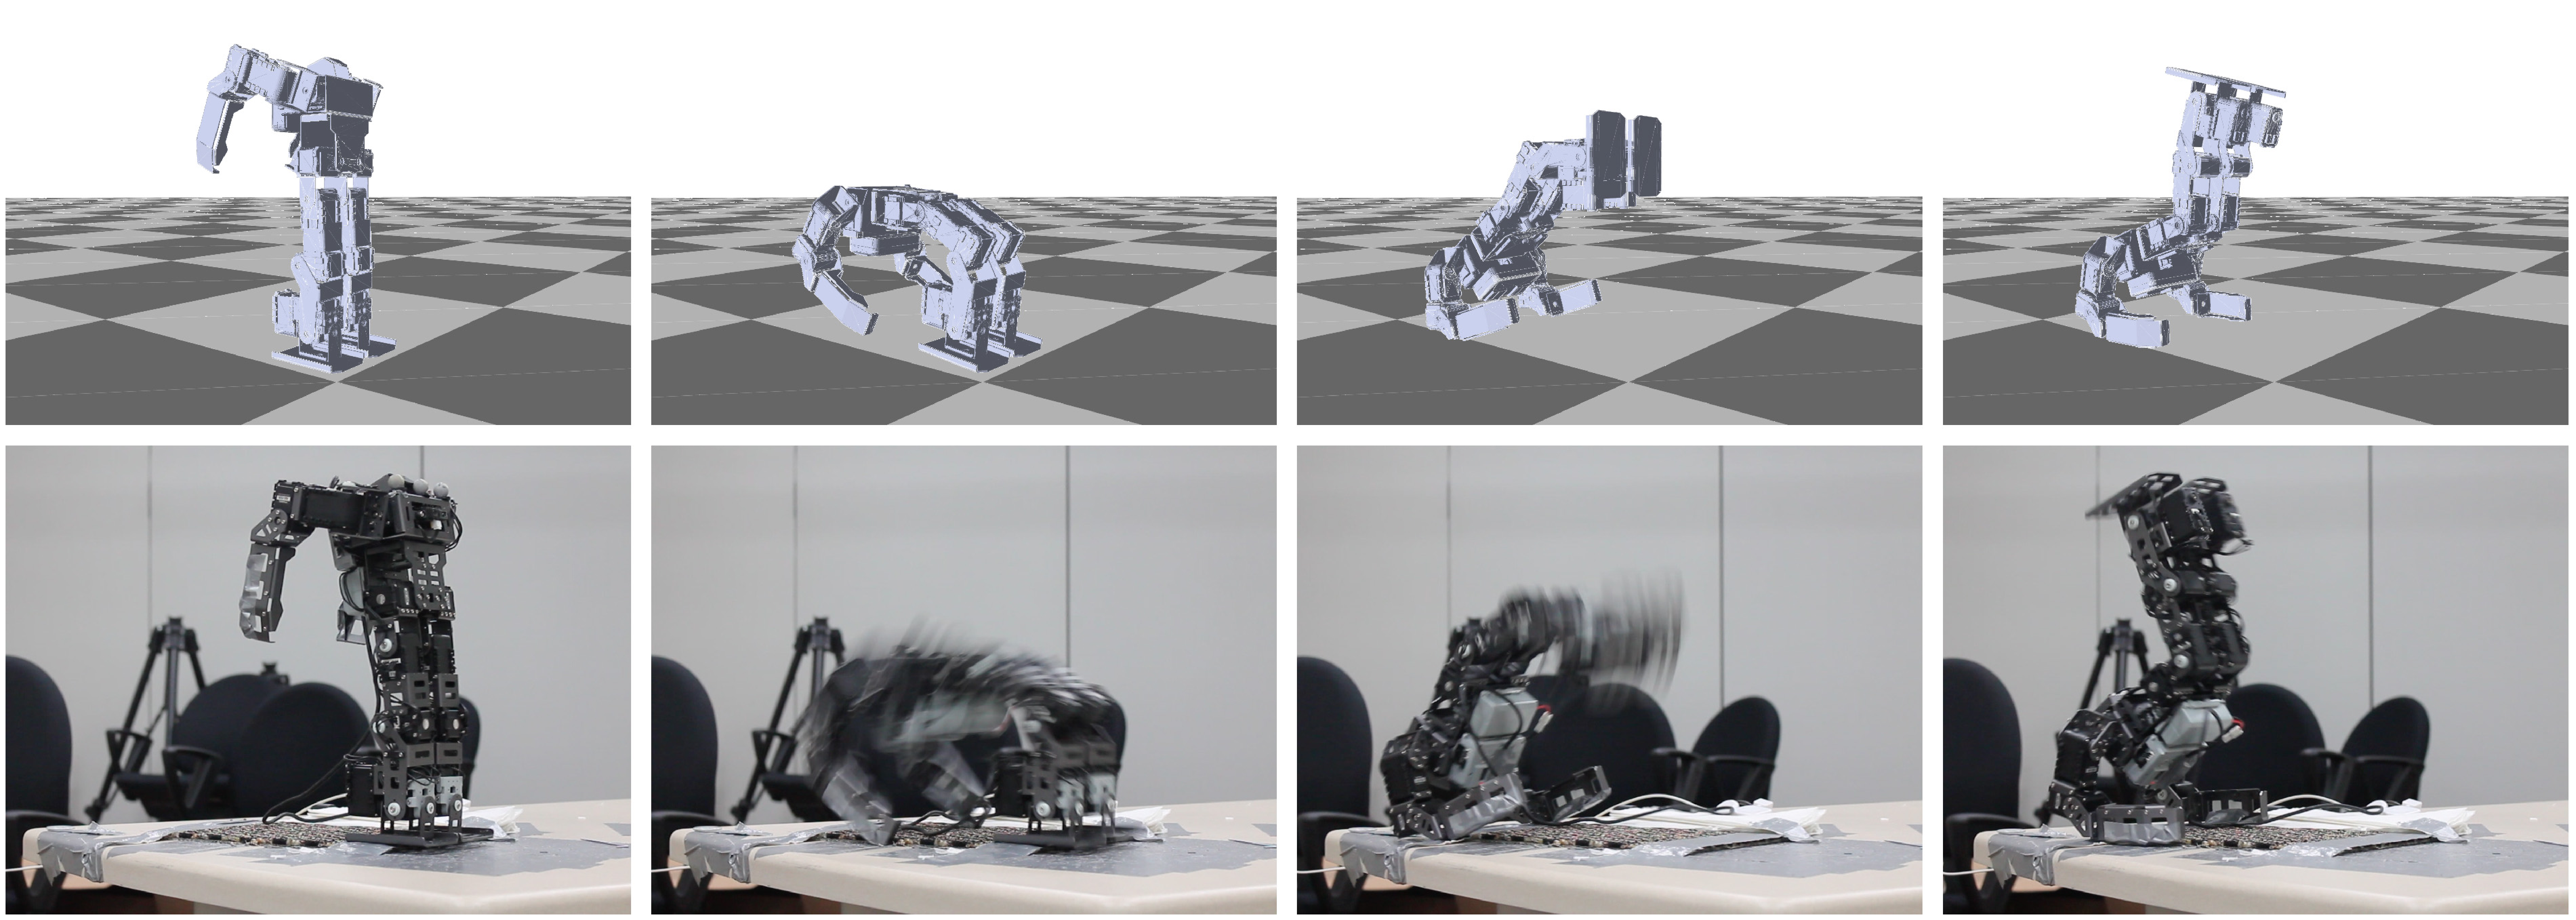
\includegraphics[width=\textwidth]{figures/stand2Hand}
  \caption{The results of the stand-to-handstand task in the simulation and on the real robot.}
  \label{fig:stand2Hand}
\end{figure*}


\subsection{Flipping to a Handstand Position}
We test our system with a more challenging task: flipping to a handstand position from a standing pose, which is often seen in gymnastics. The initial and final poses are shown in Figure~\ref{fig:stand2Hand}. The controller optimization needs to search for an additional keyframe between them. Without simulation calibration, controller optimization cannot find a controller to fulfil this task in the simulation. Nevertheless, we apply the controller with the highest fitness value to the robot to collect data for simulation calibration. After two iterations of simulation calibration and controller optimization, our system finds a successful controller that works both in the simulation and in the real world: The robot arches back rapidly and lifts its feet after the arms touch the ground. Both the speed and the curvature of the arching motion is crucial for the final balance. Although only a narrow range of such speed and curvature can lead to a balanced handstand, our system is able to automatically find a successful controller for this challenging task.


\section{Discussion}
\begin{table}
  \caption{Generalizability of the calibrated simulation}
  \vspace{-0.1in}
 \label{table:generalize}
\begin{center}
\begin{tabular}{|c|c|c|c|}
\hline
 Tasks &  I &  II  &  III \\
 \hline
 I & Succeed & Fail & Fail  \\
 II & Fail & Succeed & Fail \\
 III & Succeed & Fail & Succeed \\
 I\&II & Succeed & Succeed & Succeed\\
 I\&III & Succeed & Fail & Succeed\\
 II\&III & Succeed & Succeed & Succeed \\
 I\&II\&III & Succeed & Succeed & Succeed\\
\hline
\end{tabular}
\vspace{-0.2in}
\end{center}
 \end{table}


One important component of our system is simulation calibration. The results show that it is effective to narrow down the Reality Gap, with a minimal number of the robot experiments. In all the examples, at most two iterations of calibration (or approximately 12 seconds of robot data) is needed before we can transfer the reference trajectory to the real robot. This amount of robot data is far less than those needed in typical system identification methods.

Similar to other system identification methods, the parameters optimized in simulation calibration may not be the true physical parameters. For example, we observe that the simulation parameters optimized for the task of lean-to-stand can be different from those of kneel-to-stand. In other words, the calibrated simulator is overfitted to the current task and may not be useful for a different task. Overfitting could be a problem if the goal is to estimate the true physical parameters. However, it is not a problem in our case because the goal is to find a reference trajectory for a specific task. Actually, it is preferred because tightly coupling simulation calibration with a specific control task makes it possible to use a small amount of robot data.

One related question is how we can calibrate a simulation so that it can be generalized to other tasks. To answer this question, we perform the following two experiments. In the first experiment, we calibrate the simulation for one task (e.g. lean-to-stand) and use it to optimize a reference trajectory for a different task (e.g. sit-to-stand). We then test this trajectory on the robot. The first three rows of Table \ref{table:generalize} summarize the generalizability of the calibrated simulation when it is calibrated with a single task. Task I is lean-to-stand. Task II is sit-to-stand and Task III is kneel-to-stand. As we expected, the calibrated simulator cannot be generalized to a different task in most cases.

The second experiment is similar to the first except that we calibrate the simulation with multiple tasks (e.g. lean-to-stand and sit-to-stand). The last four rows of Table \ref{table:generalize} show that the generalizability across Task I, II and III is greatly improved if multiple tasks are used to calibrate the simulation. Multiple training tasks will improve the generalization, but they have to be similar tasks. For example, Task IV (stand-to-handstand) is drastically different from the first three tasks: It needs to maintain balance up-side-down and it experiences strong perturbations from the USB cable. If we include it in the training tasks, the results are poor.

These experiments show that if we need to design trajectories for a group of similar tasks, we may not need to perform simulation calibration for each task independently. It is likely that after developing the first few trajectories using our system, the calibrated simulation would be accurate enough. The remaining trajectories can be optimized in this simulation and further calibration is not necessary.

\section{Conclusion}

This paper has presented a complete pipeline to automatically design open loop reference trajectories for robots. This solution consists of a set of powerful computational tools: physical simulation, trajectory optimization and simulation calibration. Our system allows us to efficiently design reference trajectories of a humanoid robot to achieve four different tasks: lean-to-stand, sit-to-stand, kneel-to-stand and stand-to-handstand.

There are two venues of future work. First, we will include more simulation parameters in simulation calibration. In this paper, we have shown that adjusting the COM and the actuator gains are enough for our needs, but other simulation parameters might also be important for other tasks. A potential issue of including more simulation parameters is the increased risk of overfitting. Performing some automatic prioritizing and selection on candidate parameters would be a promising future research. Second, we believe that our system can be generalized to control other types of motions, such as walking, biking or more challenging gymnastic stunts. In these tasks, feedback control is necessary. In the future, we plan to extend our system to include feedback control and test it on a wider range of tasks.

\bibliographystyle{IEEEtran}
\bibliography{icra}

\end{document}
